\documentclass{beamer}
\usepackage[utf8]{inputenc}
\usepackage{listings}
\usetheme{Frankfurt}
\title[Pinocchio on Speed]{Pinocchio on Speed \\ Towards a dynamic, self sustainable, \\native Smaltalk implementation}
\author{Oli Flückiger}
\institute{scg.unibe.ch}
\date{May 17, 2011}

\AtBeginSection[]
{
  \begin{frame}<beamer>
    \frametitle{Layout}
    \tableofcontents[currentsection,currentsubsection]
  \end{frame}
}


%%% Smalltalkdefinition f"ur das listings-Paket
\lstdefinelanguage{Smalltalk}{
  keywordsprefix=\#,
  morekeywords={true,false,self,super,nil,thisContext}, 
  morekeywords={[2]ifTrue,ifFalse,whileTrue,whileFalse,and,or,xor,not,eqv,by,do,timesRepeat,caseOf,otherwise,withIndexDo},
  sensitive=true,
  morecomment=[s]{"}{"},
  morestring=[b]',
  moredelim=**[is][\itshape]{/+}{+/}, % benutzt f"ur tempor"are Variablen
  style=SmalltalkStyle
}
\lstdefinestyle{SmalltalkStyle}{
  tabsize=4,
%  frame=leftline,
%  frame=bl,
  framerule=2pt,
  rulecolor=\color{gray},
%  backgroundcolor=\color{white},
  backgroundcolor=\usebeamercolor[bg]{listing},
  basicstyle=\ttfamily\footnotesize,
  keywordstyle={[2]\color{gray!70!black}\bfseries},
%  stringstyle=\color{orange},
  stringstyle=\mdseries\slshape\color{gray!50!black},
%  commentstyle=\color{brown},
  commentstyle=\slshape\color{gray},
  emphstyle={\color{red}\bfseries},
  emphstyle={[2]\color{red}},
  emphstyle={[3]\color{blue}\bfseries},
  emphstyle={[4]\color{blue}},
  literate={\ _\ }{{$\gets$}}3{^}{{$\uparrow$}}1
%  literate={:=}{{$\gets$}}1{^}{{$\uparrow$}}1
%  literate={^}{{$\uparrow$}}1
} 


\begin{document}



\begin{frame}
\titlepage
\end{frame}

\begin{frame}
\begin{center}
\includegraphics[width=0.7\textwidth]{muenchhausen.png}\end{center}
\end{frame}

\section{Old Pinocchio}

\lstset{language=C}

\begin{frame}[fragile]
    \frametitle{Migrating previous codebase to a register based VM}
    \begin{lstlisting}
void op_move {
    origin = OPERAND(2);
    target = OPERAND(1);
    STORE(target, value);
    JUMP(3);
}

    ...

program_counter = &method_code;
for (;;) {
    (*program_counter)();
}
    \end{lstlisting}
\end{frame}

\section{Speed up}

\begin{frame}[fragile]
    \frametitle{Threaded execution - First prototype}
    \begin{lstlisting}

void ** pc = method->code;
goto **pc;
            
    ...

load_argument:
    origin = pc[1];
    target = pc[2];
    locals[target] = arg[origin];
    goto **( pc += 3 );

    \end{lstlisting}
\end{frame}

\begin{frame}[fragile]
    \frametitle{Mapping message sends to C functions}
    \begin{lstlisting}

int mth(Method method, void** arg) {

    register void ** sp __asm("rsp");
    alloca(method->locals * sizeof(void*));

        ...

    call_method:
        callee    = pc[1];
        arguments = pc[2]; 
        mth( sp[callee], &sp[arguments] );
        goto **( pc += 3 );

}
    \end{lstlisting}
\end{frame}

\begin{frame}[fragile]
    \frametitle{Compilers and the art of persuasion}
    {\bf Problems with compiling VMs}
    \begin{itemize}
        \item Optimizing execution inside the C code is merely guessing what the compiler might 
                actually do with the code
        \item We therefore implemented hacks to persuade GCC to compile to specific instructions, which broke again with the next modification
        \item Caching (e.g. self is always \%rbp + 1) can hurt performance
        \item Various details are crucial for speed: 
                e.g. frame pointer couldn't be ommited even though we know the frame size
    \end{itemize}
\end{frame}

\section{Kill the VM}

\begin{frame}[fragile]
    \frametitle{Observations}
    \begin{itemize}
        \item The VM had only few instructions
        \item The only complex opcodes were message sends and block evaluation
        \item JIT compilation is a (near) future goal
        \item So the behaviour of method invocation (e.g. stack usage) should match the cpu supported call/leave closely
        \item Therefore those instructions have to be implemented very specific anyway
    \end{itemize}
\end{frame}

\begin{frame}[fragile]
    \frametitle{Conclusions}
    {\bf Pinocchio self sustainable - \\Compile directly to machine code!}
    \begin{itemize}
        \item The old VM opcodes can be replaced by a few machine instructions
        \item We think the VM can be replaced completely by a compiler framework
        \item All compiler steps and all intermediate representations can 
            be implemented in a clean and polymorphic way using Smalltalk objects.
        \item Code can be written out as ELF binary which can be linked with
            arbitrary libraries.
    \end{itemize}
\end{frame}

\begin{frame}[fragile]
    \frametitle{Advantages so far...}
    {\bf Play nice with the system}
    \begin{itemize}
        \item Access to C libraries provides a generic and easy interface to the operating system
        \item And: external C functions can be linked and used to implement native functions
        \item The complete compiler framework is directly accessible within Smalltalk
        \item Rapid development progress since we can use a high level language
        \item Fast execution, less overhead than interpretation, even with semi-optimal code generation!
    \end{itemize}
\end{frame}

\section{The compiler framework}

\lstset{language=Smalltalk}

\begin{frame}[fragile]
    \frametitle{Some examples I}
    {\bf compiling a message send}
    \begin{lstlisting}

receiverTmp := receiver accept: self.
    
arguments withIndexDo: [ :arg :index |
    evaluatedArguments 
        at: index 
        put: (arg accept: self) ].
    
arguments withIndexDo: [ :arg :index |
    builder
        assign: (evaluatedArguments at: index)
        to: (self arg: index + 2 of: argsize) ].
    \end{lstlisting}
\end{frame}

\begin{frame}[fragile]
    \frametitle{Some examples I}
    {\bf compiling a message send (cont.)}
    \begin{lstlisting}
    
builder 
    assign: receiverTemp 
    to: ( self arg: 2 of: argsize ).
builder 
    indirectLoadConstant: message selector 
    into: ( self arg: 1 of: argsize ).
        
builder invoke.

ret := builder nextTemp.
builder assign: self resultVariable to: ret.

    \end{lstlisting}
\end{frame}

\begin{frame}[fragile]
    \frametitle{Some examples II}
    {\bf Developing}
    \begin{center}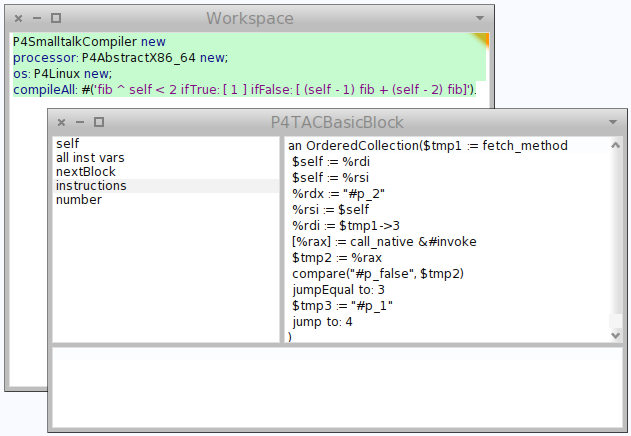
\includegraphics[width=0.9\textwidth]{developing.png}\end{center}
    hmm something is broken here. 2x self := ...
\end{frame}

\begin{frame}[fragile]
    \frametitle{Some examples III}
    {\bf allocating registers}
    \begin{lstlisting}
linearScanRegisterAllocation
  liveness do: [ :interval |
    self expireIntervalsBefore: interval start.
    (active size == self numberOfRegisters)
      ifTrue: [ self spill: interval ]
      ifFalse: [ 
        self nextFreeRegisterFor: interval variable.  
        active add: interval ]].
    \end{lstlisting}
\end{frame}


\section{The Runtime}

\begin{frame}[fragile]
    \frametitle{Down to business}
    \begin{itemize}
        \item Compiling a Method:
        \begin{itemize}
            \item Parser generates AST
            \item Generate TAC, inlineing some control constructs (ifTrue, while)
            \item Conservative liveness analysis
            \item Linear Scan Register Allocation
            \item Postcompilation, optimizations
            \item Assembling
            \item Writing out ELF
            \item Linking
        \end{itemize}
        \item Running the generated binary:
        \begin{itemize}
            \item Loading the code, exporting symbols, loading global literals (done by the kernel)
            \item Run initialization method loading Objects into memory
        \end{itemize}
        \item The loaded code itself could include the compiler, therefore beeing able to modify code, write out another ELF file or an image
    \end{itemize}
\end{frame}

\begin{frame}[fragile]
    \frametitle{Memory Layout}
    {\bf Memory layout }
    \begin{center}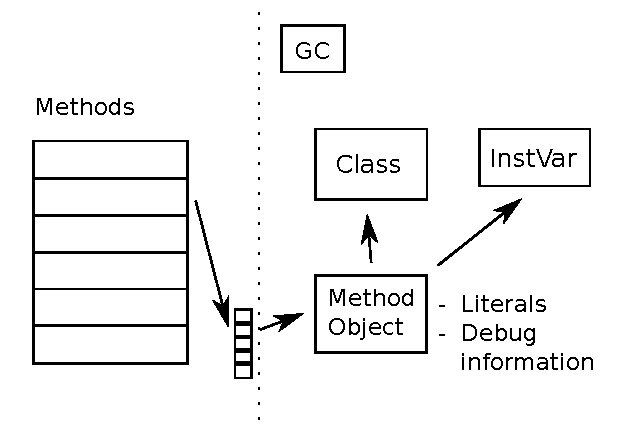
\includegraphics[width=0.9\textwidth]{memory.pdf}\end{center}
\end{frame}

\begin{frame}[fragile]
    \frametitle{The main idea}
    {\bf All parts of this puzzle should be implemented by normal Smalltalk objects: }
    \begin{itemize}
        \item Compiler
        \item Assembler
        \item Object Layouts
        \item MethodDictionary
        \item Garbage Collector
        \item (Integers)
        \item Anything.... 
    \end{itemize}
\end{frame}

\begin{frame}[fragile]
    \frametitle{Late bound variables}
    {\bf self inspect: foo }
    \begin{itemize}
        \item What is foo?
        \item Class can only be determined at runtime! 
        \item (Almost) everything is late bound in Smalltalk
    \end{itemize}
\end{frame}

\section{To boldly go where...}

\begin{frame}{How Pinocchio runs itself}

    {\bf MethodDictionary methodDictionary at: \#at}

    \begin{center}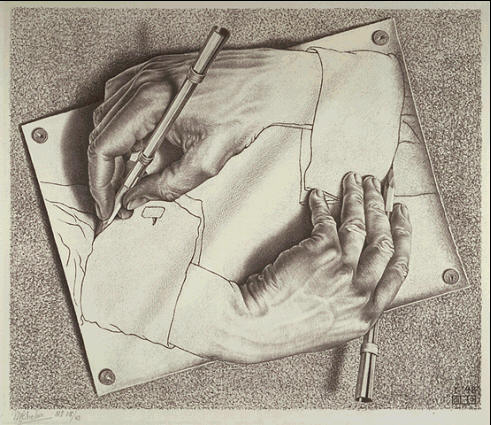
\includegraphics[width=0.7\textwidth]{escher.jpg}\end{center}
\end{frame}

\begin{frame}[fragile]
    \frametitle{Inline caches}

    \begin{lstlisting}
(callee class == MethodDictionary)
    ifTrue: [ <invoke #MethodDictionary_at> ]
    ifFalse: [ callee at: arg ]
    \end{lstlisting}

    \begin{itemize}
        \item Inline caches store predictions about the callees class directly inside the callers code
        \item Pointer to the predicted target code is inlined to avoid pipeline stalls
    \end{itemize}
\end{frame}

\lstset{language=C}

\begin{frame}[fragile]
    \frametitle{More on inline caches}

    {\bf Sketched implementation of a polymorphic inline cache at assembler level}

    \begin{lstlisting}

add:
1:    ( callee_class == Integer   )   call: &1234
2:    ( callee_class == Character )   call: &1235
3:    ( callee_class == String    )   call: &1236
4:      "empty inline cache"

      jump: &invoke_method

invoke_method:
      address = lookup( callee_class, add )
      add_inline_cache( caller, 4, callee_class, address )
      call: &address

    \end{lstlisting}

\end{frame}

\begin{frame}{JIT implementation made easy}
        \begin{itemize}
            \item Determine a often used inline cache
            \item Compile the called method using the new gained type information about the callee
            \item Replace the address of this method with native code
        \end{itemize}
\end{frame}

\begin{frame}{From late to early bound}

    {\bf Natives are just hardwired inline caches with native code generated by the JIT compiler}
    \begin{itemize}
            \item A MethodDictionary can therefore be implemented by simply hardwiring the inline cache for \#at
            \item The \#at method should be compiled assumeing that self always reffers to the current implementation of this particular MethodDictionary
            \item This ''freezes'' the method in its current state and generates fast native code
            \item The runtime can do a dictionary lookup without ending up in a self referential loop
            \item But the implementation doesn't loose its polymorphic behaviour: any MethodDictionary can be replaced by a subclass and almost everything works as expected!
    \end{itemize}
\end{frame}
\end{document}
